%======================================================================
\NEWSEC
%======================================================================

\subsection{\ssLoadBalance}

\begin{frame}[fragile,label=ss-load-balance] 
\secframetitle{\ssLoadBalance}
\footnotesize
\begin{tabbing}
xxxxxx\=xxxxxx\=xxxxxx\=\kill
\bluecode{Balance \{} \\
\>     \code{schedule \{} \\
\>\>   \code{var = }\bluecode{"cycle"}\code{;}\\
\>\>   \bluecode{step  = 100;} \\
\> \} \\
\}
\end{tabbing}
\begin{semiverbatim}
\uncover<2->{\prompt \redcode{charmrun +p4 bin/enzo-p input/load-balance-4.in }\bluecode{+balancer RefineLB}}\cursor{2}
\end{semiverbatim}
\uncover<3->{\urltext{http://charm.cs.illinois.edu/manuals/html/charm++/7.html} \\
\textit{``The commonly used load balancers include }\bluecode{BlockLB}
\bluecode{ComboCentLB},
\bluecode{CommLB},
\bluecode{DistributedLB},
\bluecode{DummyLB},
\bluecode{GreedyCommLB},
\bluecode{GreedyLB},
\bluecode{HybridLB},
\bluecode{NeighborLB},
\bluecode{OrbLB},
\bluecode{RandCentLB},
\bluecode{RefineCommLB},
\bluecode{RefineLB},
\bluecode{RefineSwapLB},
\bluecode{RotateLB}.''}
\end{frame}

%----------------------------------------------------------------------

\begin{frame}[fragile]
\secframetitle{\ssLoadBalance}
\begin{center}
\begin{minipage}{1.3in}

\includegraphics[width=1.3in]{Images/Balance/balance-de-00000.png}
\end{minipage}
\begin{minipage}{1.3in}
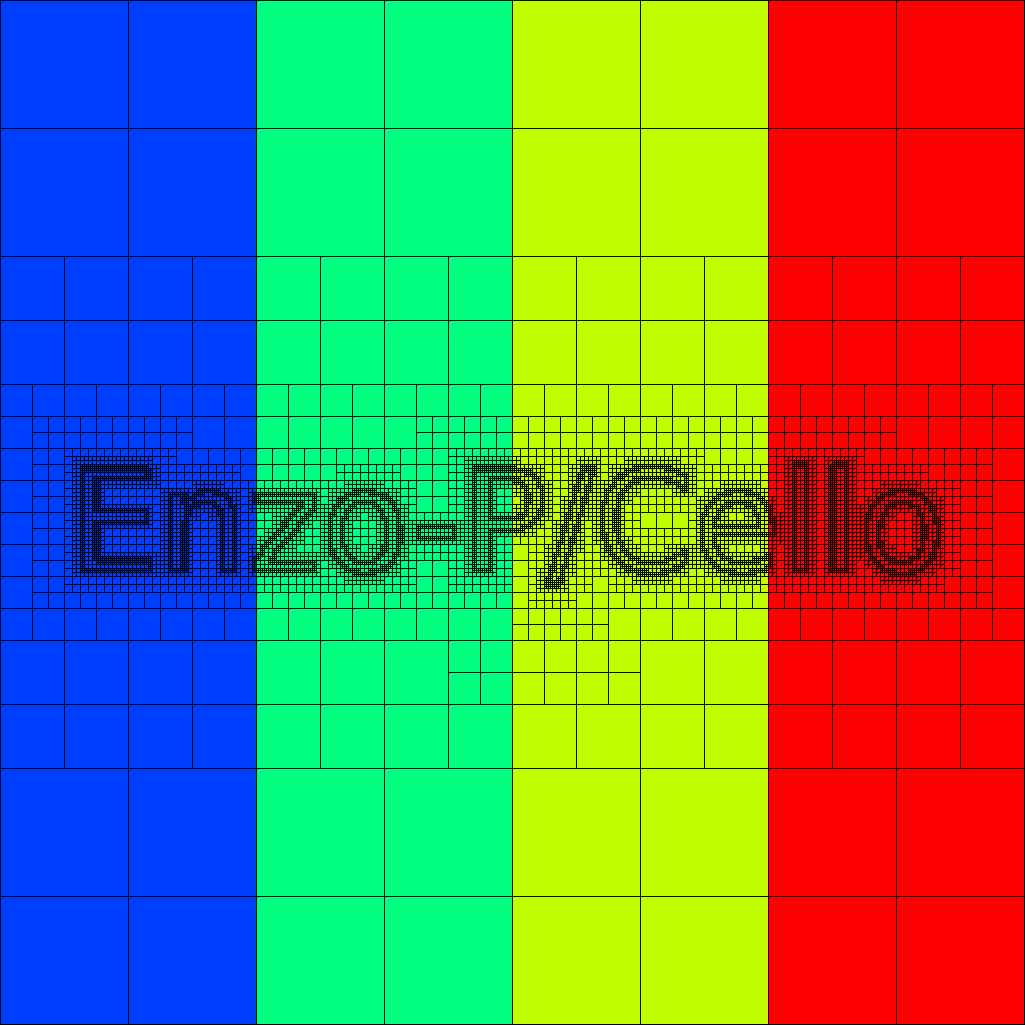
\includegraphics[width=1.3in]{Images/Balance/balance-mesh-00000.png}
\end{minipage}
\begin{minipage}{1.3in}
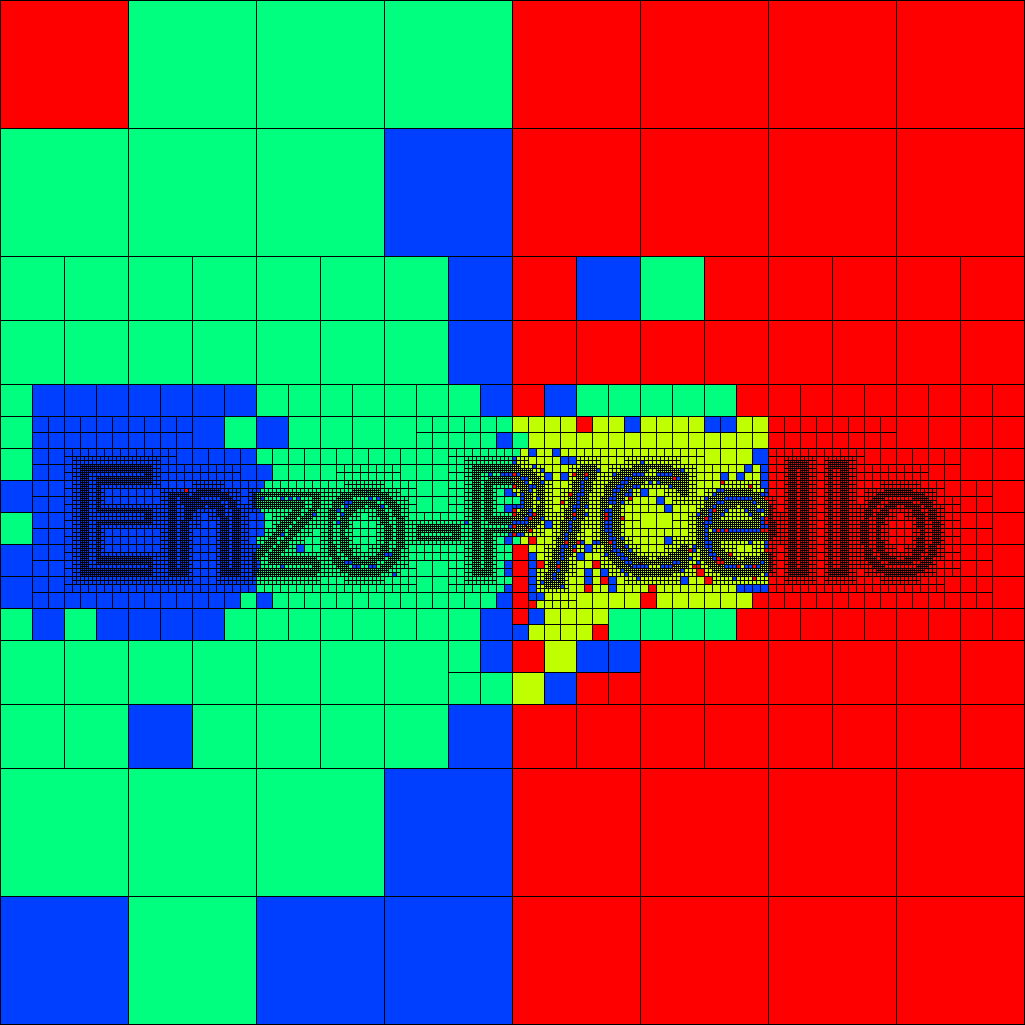
\includegraphics[width=1.3in]{Images/Balance/balance-mesh-00002.png}
\end{minipage}
\begin{minipage}{1.3in}
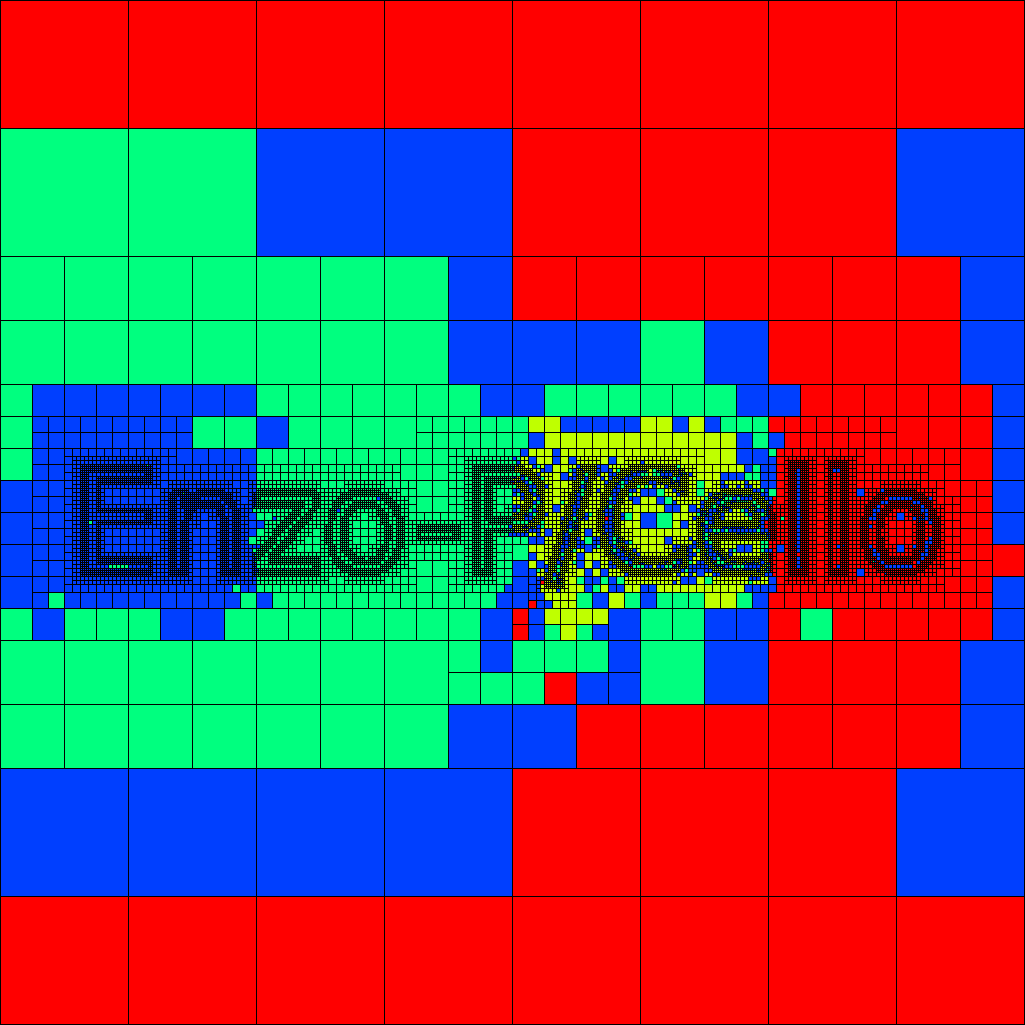
\includegraphics[width=1.3in]{Images/Balance/balance-mesh-00004.png}
\end{minipage}
\begin{minipage}{1.3in}
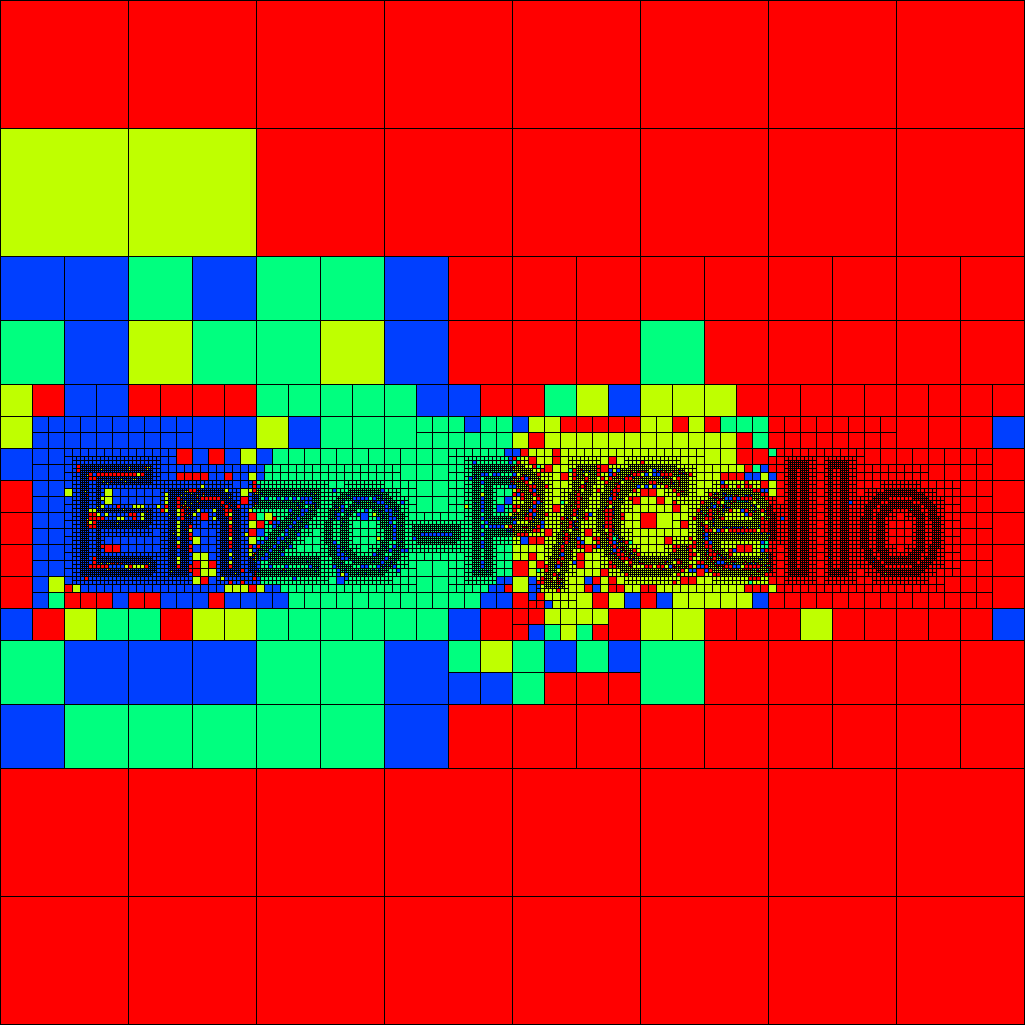
\includegraphics[width=1.3in]{Images/Balance/balance-mesh-00006.png}
\end{minipage}
\begin{minipage}{1.3in}
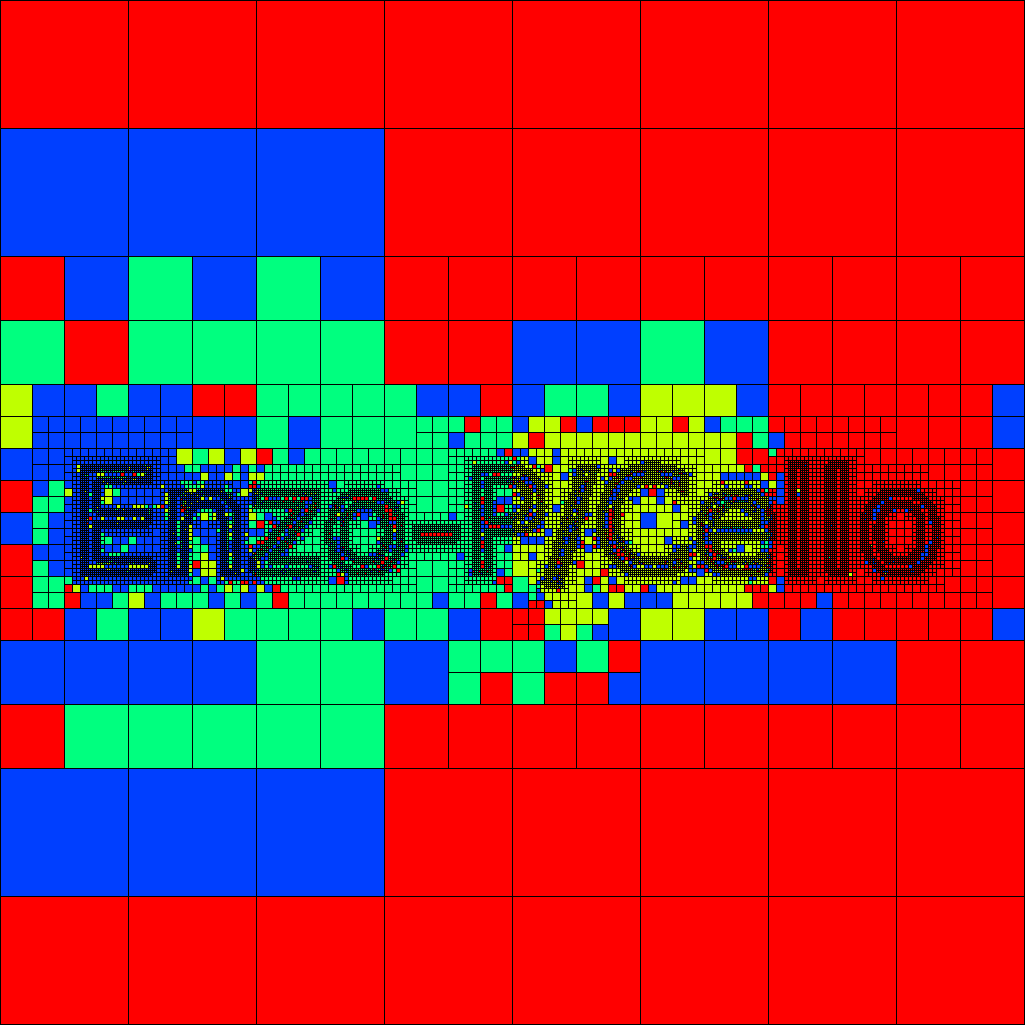
\includegraphics[width=1.3in]{Images/Balance/balance-mesh-00008.png}
\end{minipage}
\end{center}
\end{frame}
%----------------------------------------------------------------------



%     ComboCentLB : A special load balancer that can be used to combine any number of centralized load balancers mentioned above.

%     GreedyCommLB : Extends the greedy algorithm to take the communication graph into account.
%     GreedyLB : Uses a greedy algorithm that always assigns the heaviest object to the least loaded processor.
%     MetisLB : Uses METIS TM to partitioning object communication graph.
%     RandCentLB : Randomly assigns objects to processors;
%     RefineCommLB : Same idea as in RefineLB, but takes communication into account.
%     RefineLB : Moves objects away from the most overloaded processors to reach average, limits the number of objects migrated.
%     RefineSwapLB : Moves objects away from the most overloaded processors to reach average. In case it cannot migrate an object from an overloaded processor to an underloaded processor, it swaps objects to reduce the load on the overloaded processor. This strategy limits the number of objects migrated.
%     RefineTopoLB : Same idea as in RefineLB, but takes processor topology into account.
%     TopoCentLB : Extends the greedy algorithm to take processor topology into account.
